\begin{figure}[ht]
\centering
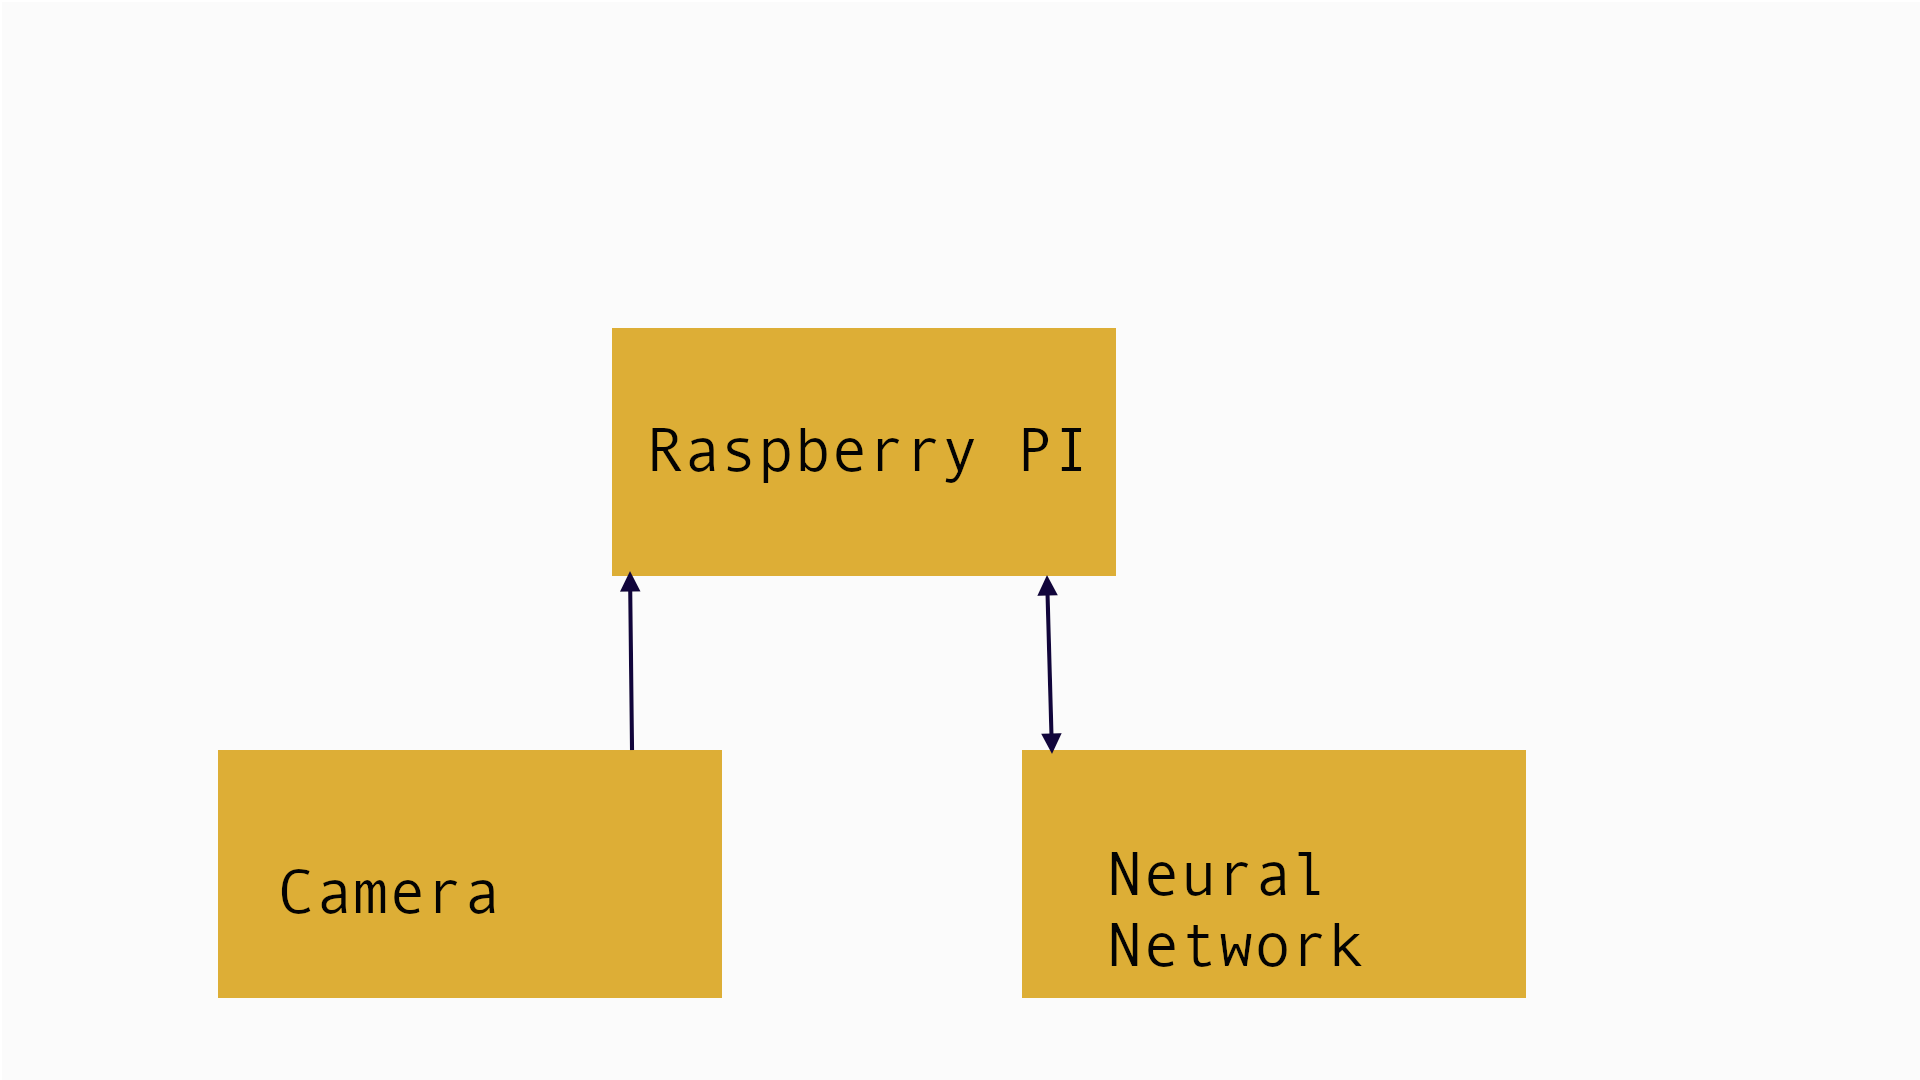
\includegraphics[scale=0.7]{block}
\caption{Different components of attention tracker}
\end{figure}

\section{Raspberry PI}
The Raspberry PI is a small single-board computer. It is developed by Raspberry PI Foundation to promote teaching of basic computer science in schools. It has  1.2 GHz 64-bit quad core processor, on-board 802.11n Wi-Fi, Bluetooth and USB boot capabilities. 

\section{Image Processing}
Neural network includes Image preprocessing block, feature extraction block and an implementation of deep learning network. Image processing works by convering the given image to integral image.

\subsection{Neural Network}
Neural network is a series of weigted functions. These functions give output based on the threshold function. The threshold function can be softmax or spiking neural network etc.  This can be used to detect features
of image which can determine whether a given image has a face or not. This is done by
training neural network on known images, which have faces and adjusting weights to reduce false positives. In put to neural network is an integral image. Which is better
at detecting face than traditional methods like primary component vector analysis, which operate on entire image.
\subsection{Integral Image}
Integral image is the concept introduced by Viola Jones et al. It makes image processing faster. It is done by subjecting all the pixels of image to the following set of transformations.
\begin{align*}
    IntegralImage(x,y) &=Image(x,y)+IntegralImage(x-1,y)+IntegralImage(x,y-1)\\
    IntegralImage(x,-1) &=0\\
    IntegralImage(-1,0) &=0\
\end{align*}
The resulting $IntegralImage$ makes it faster to perform image detection functions like the Haar Function. The Haar function selects rectangular regions in an image, and finds their difference from other rectangular region.
\begin{figure}[ht]
\centering
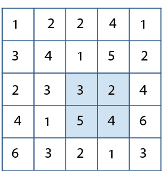
\includegraphics[scale=0.7]{image}
\caption{image with pixels represented by numbers}
\end{figure}

\begin{figure}[ht]
\centering
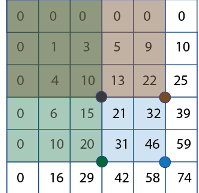
\includegraphics[scale=0.7]{iimage}
\caption{integral image}
\end{figure}


